\documentclass[a4page]{article}

\usepackage[english]{babel}
\usepackage[utf8]{inputenc}
\usepackage{amsmath}
\usepackage{bm}
\usepackage{float}
\usepackage{xfrac}
\usepackage{graphicx}
\graphicspath{ {./figures/} }
\usepackage{setspace}
\usepackage{listings}
\usepackage[colorinlistoftodos]{todonotes}
%\onehalfspacing
%\doublespacing
\title{STAT3016 Final Project}

\author{Dong Luo\\ u5319900}

\date{\today}

\begin{document}
	\maketitle
	\section{Introduction}
	Linear regression is widely used in data analysis of various fileds. In this project, we will be exploring several Bayesian techniques to fit and analysis linear regression models.\\
	The dataset set we will be using in this project will solely be the \textit{Bank Marketing Campaign Data Set} provided on the STAT3016 course website. This dataset is the outcome of direct marketing campaigns of a Portuguese banking institution through phone calls.\\
	The dataset contains the personal information of 45211 contacts, and the main point we are interested in is whether the balance depends on the contacts' marital status. Specifically, we want to know if the balance of contacts differs between those who are single, married and divorced. We will also assume that the contacts' age and whether one has a house loan may affect the balance.\\
	The subset of dataset we will be using includes the attribute balance, age, housing, and marital as they are assumed to be the potential predictors and response variables in the linear regression model. Other attributes will be ignored in this project, even though some of them, such as education, are likely to have influence on the balance. The limitations of we excluding other potential predictors will be discussed in section \ref{Self-Criticism}.

%*******************************************************
%******************    Section 2    ********************
%*******************************************************

	\section{Methodology}
	\subsection{Model Comparison\label{2.1}}
	Assuming the relationship between balance and age to be linear, the regressors may include the three main effects (age, house, and marital), all two-way interactions and the three-way interaction.\\
	When fitting an ordinary least squares (OLS) regression, we can just use the \verb|lm()| function in R and then analysis the significance level of each term:
	\begin{verbatim}
        lm(balance~age*housing*marital)
    \end{verbatim}
	In Bayesian approach, we will use the parametrisation below (introduced in Section 9.3.1 of Hoff):
	\begin{equation}
	y_i=z_1b_1x_{i,1}+\dots+z_pb_px_{i,p}+\epsilon_i,\label{parametrisation}
	\end{equation}
	where $z_j$ indicates whether the regression coefficient of the $j^{th}$ predictors is zero.\\
	As the `marital status' is a factor variable of 3 levels, we will need $3-1=2$ indicator(dummy) variables. Similarly, we need $2-1=1$ indicator variable for the factor variable `housing', which has two levels. Hence, there will be $1+2+1=4$ terms for main effects, $1\times2+1\times1+2\times1=5$ terms for two-way interactions, $1\times2\times1=2$ terms for the three-way interaction, and a term for the intercept. Using the parametrisation in equation \ref{parametrisation}
	, our linear regression model will look like
	\begin{equation}
	y_i=z_1b_1x_{i,1}+z_2b_2x_{i,2}+\dots+z_{12}b_{12}x_{i,12}+\epsilon_i,\label{full-model}
	\end{equation}
    where\\
	$x_{i,1}=1$ for each subject $i$\\
	$x_{i,2}=$ age of subject $i$\\
	$x_{i,3}=1$ if subject $i$ is single, 0 otherwise\\
	$x_{i,4}=1$ if subject $i$ is married, 0 otherwise\\
	$x_{i,5}=1$ if subject $i$ has house loan, 0 if not\\
	$x_{i,6}=x_{i,2}\times x_{i,5}$\\
	$x_{i,7}=x_{i,2}\times x_{i,3}$\\
	$x_{i,8}=x_{i,2}\times x_{i,4}$\\
	$x_{i,9}=x_{i,3}\times x_{i,5}$\\
	$x_{i,10}=x_{i,4}\times x_{i,5}$\\
	$x_{i,11}=x_{i,2}\times x_{i,3}\times x_{i,5}$\\
	$x_{i,11}=x_{i,2}\times x_{i,4}\times x_{i,5}$.\\
	When we include a two-way interaction term, we usually have to include both main effects of the two predictors. Similarly, we have to include all corresponding main effects and two-way interactions before we can include the three-way interaction term in the model. Therefore, we will consider a total of 18 possible models, shown in the table \ref{table-z}.
    \begin{center}
        \begin{table}[H]
            \begin{tabular}{c|c||c|c}  
                model index&\textbf{z}&model index&\textbf{z}\\
                \hline
                1 & (1,0,0,0,0,0,0,0,0,0,0,0)&10&	(1,1,0,0,1,1,0,0,0,0,0,0)	\\ 
                2 & (1,1,0,0,0,0,0,0,0,0,0,0)&11&	(1,1,1,1,1,0,0,0,0,0,0,0)	\\
                3 & (1,0,1,1,0,0,0,0,0,0,0,0)&12&	(1,1,1,1,1,1,0,0,0,0,0,0)	\\
                4 & (1,0,0,1,1,0,0,0,0,0,0,0)&13&	(1,1,1,1,1,0,1,1,0,0,0,0)	\\
                5 & (1,1,1,1,0,0,0,0,0,0,0,0)&14&	(1,1,1,1,1,0,0,0,1,1,0,0)	\\
                6 &	(1,0,1,1,1,0,0,0,0,0,0,0)&15&	(1,1,1,1,1,1,1,1,0,0,0,0)	\\
                7 &	(1,1,0,0,1,0,0,0,0,0,0,0)&16&	(1,1,1,1,1,1,0,0,1,1,0,0)	\\
                8 &	(1,1,1,1,0,0,1,1,0,0,0,0)&17&	(1,1,1,1,1,0,1,1,1,1,0,0)	\\
                9 &	(1,0,1,1,1,0,0,0,1,1,0,0)&18&	(1,1,1,1,1,1,1,1,1,1,1,1)	\\	
            \end{tabular}
        \caption{The candidate models and their $\bm{z}$'s}
        \label{table-z}
        \end{table}
    \end{center}
	We can then compare the candidate models above by their marginal probabilities:
	\begin{equation}
	p(\bm{z}|\bm{y},\bm{X})\propto p(\bm{z})p(\bm{y}|\bm{X},\bm{z}).\label{marginalp1}
	\end{equation}
	Without much extra information, we may assume a discrete uniform prior for $z$. Hence the equation \ref{marginalp1} becomes:
	\begin{equation}
	\begin{split}
	p(\bm{z}|\bm{y},\bm{X})&\propto p(\bm{z})p(\bm{y}|\bm{X},\bm{z})\\
	&\propto p(\bm{y}|\bm{X},\bm{z}).\label{marginalp2}
	\end{split}
	\end{equation}
	The equation for computing $p(\bm{y}|\bm{X},\bm{z})$, when we assume a $g$-prior for $\bm{\beta}$ and inverse gamma prior for $\sigma^2$ with parameters $(\nu_0/2,\nu_0\sigma_0^2/2)$, is given in page 165 of Hoff:
	\begin{equation}
	p(\bm{y}|\bm{X},\bm{z})=\pi^{-n/2}\frac{\mathit{\Gamma}([\nu_0+n]/2)}
		{\mathit{\Gamma}(\nu_0/2)}(1+g)^{-p_z/2}
		\frac{(\nu_0\sigma_0^2)^{\nu_0/2}}
		{(\nu_0\sigma_0^2+\text{SSR}_g^z)^{(\nu_0+n)/2}},\label{marginalp3}
	\end{equation}
	where $\text{SSR}_g^z$ is:
	\begin{equation}
	\text{SSR}_g^z=\bm{y}^T(\textbf{I}-\frac{g}{g+1}\textbf{X}_z(\textbf{X}_z^T\textbf{X}_z)^{-1}\textbf{X}_z^T)\bm{y}
	\label{SSR1}
	\end{equation}
	We set $g=n$ and use the unit information prior for $p(\sigma^2)$ for each model $\bm{z}$ as what the textbook (Hoff) does.
	When we tried computing $\log p(\bm{y}|\bm{X},\bm{z})$ using the \verb|lpy.X| provided in \verb|regression_gprior.r|, the following error occurred:
	\begin{singlespace}
		\begin{verbatim}
> lpy.X(y,X[,z[1,],drop=FALSE])
Error: cannot allocate vector of size 15.2 Gb
In addition: Warning messages:
1: In lpy.X(y, X[, z[1, ], drop = FALSE]) :
Reached total allocation of 8051Mb: see help(memory.size)
		\end{verbatim}
	\end{singlespace}
	Clearly, a matrix of size 15.2 Gb is too large for most computers to perform computation with. The large matrix is generated during the calculation of $SSR_g^z$. In equation \ref{SSR1},  $\textbf{X}_z(\textbf{X}_z^T\textbf{X}_z)^{-1}\textbf{X}_z^T$ is a 45211 by 45211 matrix as $\textbf{X}_z$ has 45211 rows and 
	$\textbf{X}_z^T$ has 45211 columns. To avoid creating such large matrices, we can expand equation \ref{SSR1} and by applying dynamic programming techniques, we get the following rearrangement:
	\begin{equation}
	\begin{split}	
	\text{SSR}_g^z
	&=\bm{y}^T(\textbf{I}-\frac{g}{g+1}\textbf{X}_z(\textbf{X}_z^T\textbf{X}_z)^{-1}\textbf{X}_z^T)\bm{y}\\
	&=\bm{y}^T\bm{y}-\frac{g}{g+1}\bm{y}^T\textbf{X}_z(\textbf{X}_z^T\textbf{X}_z)^{-1}(\textbf{X}_z^T\bm{y}),
	\label{SSR2}
	\end{split}
	\end{equation}
	which minimises the number of scaler multiplications and does not create huge matrices.\\
	After getting $\log p(\bm{y}|\bm{X},\bm{z}_i)$ for each model $\bm{z}_i$, we want to get $p(\bm{z}_i|\bm{y},\bm{X}) = \dfrac{\exp(\log p(\bm{y}|\bm{X},\bm{z}_i))}{\sum_j \exp(\log p(\bm{y}|\bm{X},\bm{z}_j))}$. As the dataset is large, the log-likelihood, $\log p(\bm{y}|\bm{X},\bm{z})$, computed for all models are less than -426510, which are relatively small. Simply computing $\exp(\log p(\bm{y}|\bm{X},\bm{z}))$ would result in 0's for all model $\bm{z}$. As
	\begin{equation}
	\begin{split}	
	p(\bm{z}_i|\bm{y},\bm{X}) 
	&= \frac{\exp(\log p(\bm{y}|\bm{X},\bm{z}_i))}{\sum_j \exp(\log p(\bm{y}|\bm{X},\bm{z}_j))}\\
	&= \frac{\sfrac{\exp(\log p(\bm{y}|\bm{X},\bm{z}_i))}{exp(c)}}{\sfrac{\sum_j \exp(\log p(\bm{y}|\bm{X},\bm{z}_j))}{exp(c)}}\\
	&= \frac{\sfrac{\exp(\log p(\bm{y}|\bm{X},\bm{z}_i))}{exp(c)}}{\sum_j \dfrac{ \exp(\log p(\bm{y}|\bm{X},\bm{z}_j))}{exp(c)}}\\
	&= \frac{\exp(\log p(\bm{y}|\bm{X},\bm{z}_i) - c)}{\sum_j \exp(\log p(\bm{y}|\bm{X},\bm{z}_j) - c)}
	\label{lpy.p}
	\end{split}
	\end{equation}
	for any real number $c$. We may let $c$ be the mean $\left(\text{i.e. } \frac{\sum_{j=1}^n \log p(\bm{y}|\bm{X},\bm{z}_j)}{n}\right)$, where $n$ is the number of candidate models.
	\subsection{Model Averaging\label{2.2}}
	In section \ref{2.1}, we proposed 18 potential models to be compared while we only used three variables from the dataset to make regressors. The dataset we are using contains a total of 16 variables besides balance. Hence we may have $2^{17}$ potential models, and possibly much more when we consider possible interaction terms and quadratic terms. The number of potential models grows exponentially as the we have more covariates. It would be inefficient to compute $p(\bm{z}_i|\bm{y},\bm{X})$ for each $\bm{z}_i$ to find models of high marginal probabilities.\\
	One more efficient way to compare models is model averaging. We implement a Gibbs sampler to approximate the posterior probabilities of $\bm{z}\ (\text{i.e. }p(\bm{z}|\bm{y},\bm{X}))$. In iteration $s$ of the Gibbs sampler, we generate $z_j^{(s)}$ by sampling from $p(z_j|\bm{y},\bm{X},\bm{z}_{-j})$, where $\bm{z}_{-j}$ stands for all $z_i$'s in $\bm{z}$ such that $i\neq j$.\\
	Assume discrete uniform prior for each $z_j$ such that $Pr(z_j=1)=Pr(z_j=0)=0.5$. We can compute $p(z_j|\bm{y},\bm{X},\bm{z}_{-j})$ as
	\begin{equation}
		\begin{split}
		Pr(z_j=1|\bm{y},\bm{X},z_{-j})
		&=\frac{Pr(z_j=1|\bm{y},\bm{X},z_{-j})}{1}\\
		&=\frac{Pr(z_j=1|\bm{y},\bm{X},z_{-j})}{Pr(z_j=1|\bm{y},\bm{X},z_{-j})+Pr(z_j=0|\bm{y},\bm{X},z_{-j})}\\
		&=\frac{1}{1+\dfrac{Pr(z_j=0|\bm{y},\bm{X},z_{-j})}{Pr(z_j=1|\bm{y},\bm{X},z_{-j})}}\\
		&=\frac{1}{1+\dfrac{Pr(z_j=0)}{Pr(z_j=1)}\times\dfrac{p(\bm{y}|\bm{X},\bm{z}_{-j},z_j=0)}{p(\bm{y}|\bm{X},\bm{z}_{-j},z_j=1)}}\\
		&=\frac{1}{1+\dfrac{p(\bm{y}|\bm{X},\bm{z}_{-j},z_j=0)}{p(\bm{y}|\bm{X},\bm{z}_{-j},z_j=1)}}\\
		&=\frac{1}{1+ \exp (\log p(\bm{y}|\bm{X},\bm{z}_{-j},z_j=0) - \log p(\bm{y}|\bm{X},\bm{z}_{-j},z_j=1))}.
		\end{split}
	\end{equation}
	The \verb|lpy.X| function from \verb|regression_gprior.r| by Hoff is used to compute $\log p(\bm{y}|\bm{X},\bm{z})$ for different $\bm{z}$'s. The R code for the Gibbs sampler is:
\begin{verbatim}
##### Starting values and MCMC setup
z<-rep(1,ncol(X))#Starting value for z
lpy.c<-lpy.X3(y[subset],X[subset,z==1,drop=FALSE])
S<-10000
Z<-matrix(NA,S,ncol(X))

##### Gibbs sampler
for(s in 1:S){
    for(j in sample(2:dim(X)[2])){
        zp<-z;
        zp[j]<-1-zp[j]
        lpy.p<-lpy.X3(y,X[,zp==1,drop=FALSE])
        r<-(lpy.p-lpy.c)*(-1)^(zp[j]==0)
        z[j]<-rbinom(1,1,1/(1+exp(-r)))
        if(z[j]==zp[j]){
            lpy.c<-lpy.p
        }
    }
    Z[s,]<-z
}
\end{verbatim}
	In the loop for generating $z_j$'s, we never generate a $z_1$ as we always want the intercept in a linear regression.\\
	As the generation of $\bm{z}$ in the above code does not depend on $\beta$. We can generate posterior samples of $\beta$ using the MCMC draws of $\bm{z}$'s stored in \verb|Z|.
    \begin{verbatim}
BETA<-matrix(NA,S,ncol(X))
for(i in 1:nrow(Z)){
    beta<-Z[i,]
    beta[Z[i,]==1]<-lm.gprior3(y,X[,Z[i,]==1,drop=FALSE],S=1)$beta
    BETA[i,]<-beta
}
    \end{verbatim}
	The \verb|lm.gprior3| function in the above code is just the \verb|lm.gprior| by Hoff with slight modification (modified the part computing $SSR$, mentioned in \ref{2.1}). In each iteration \verb|i|, we draw a $\beta$ from the its (conditional) posterior distribution using the columns of \verb|X| whose corresponding $z_j$'s are $1$'s.\\
	When we were constructing the matrix \verb|X|, we let it have 12 rows which stands for the 12 regressors (including the intercept):
	\begin{verbatim}
		> colnames(X)
		[1] ""                    "age"                 "m.single"           
		[4] "m.married"           "h.yes"               "age_h.yes"          
		[7] "age:m.single"        "age:m.married"       "m.single:h.yes"     
		[10] "m.married:h.yes"     "age:m.single:h.yes"  "age:m.married:h.yes"
	\end{verbatim}
	Notice that the $3^{\text{th}}$ and the $4^{\text{th}}$ are two dummy variables of the factor \verb|matiral|. The posterior distribution of $p(z_3|\bm{y},\bm{X})$ and $p(z_4|\bm{y},\bm{X})$ are often different. This is because the effects of some levels may significantly differ from others, and the effects may looks similar between some pair of levels.\\
	We want to know the significance of \verb|marital| rather than a particular level as we usually either put in the variable (all levels) or don't when examining a predictor variable of multiple levels. Therefore, we can improve the model averaging process by "grouping" the two dummy variables (i.e. we either set both to 1 or to be 0 in each iteration), and we do the same thing for the interaction terms:
    	\begin{verbatim}
##### Starting values and MCMC setup
g<-list(2,c(3,4),5,6,c(7,8),c(9,10),c(11,12))
z<-rep(1,ncol(X))
lpy.c<-lpy.X3(y,X[,z==1,drop=FALSE])
S<-10000
Z2<-matrix(NA,S,ncol(X))
BETA2<-matrix(NA,S,ncol(X))

#####Gibbs sampler
for(s in 1:S){
    for(j in sample(1:length(g))){
        zp<-z; zp[g[[j]]]<-1-zp[g[[j]]]
        lpy.p<-lpy.X3(y,X[,zp==1,drop=FALSE])
        r<-(lpy.p-lpy.c)*(-1)^(zp[g[[j]]][1]==0)
        z[g[[j]]]<-rep(rbinom(1,1,1/(1+exp(-r))),length(g[[j]]))
        if(z[g[[j]]][1]==zp[g[[j]]][1]){
            lpy.c<-lpy.p
        }
    }
    Z2[s,]<-z
}

for(i in 1:nrow(Z2)){
    beta<-Z2[i,]
    beta[Z2[i,]==1]<-lm.gprior3(y,X[,Z2[i,]==1,drop=FALSE],S=1)$beta
    BETA2[i,]<-beta
}
    \end{verbatim}
    
    In each iteration, the inner for loop is executed 7 times for the 7 "partitions" of the $\bm{z}$ vectors, including three main effects, three two-way interactions, and a three-way interaction. Each partition is represented as an element in the list \verb|g|, and \verb|sample(1:length(g))| makes the order of partitions of $\bm{z}$ to be updated to be random in each iteration.\\
    In such way, we ensures that the approximated $p(z_j|\bm{y},\bm{X})$'s are the same for all $z_j$'s in one partition of $z$. Thus, we are able to decide whether a factor variable or a interaction term involving a factor variable is significant in the regression model.
	
	\section{Results \label{results}}
	The result of model comparison in section \ref{2.1} is as follows:
    \begin{verbatim}
> sort(round(exp(-mean(lpy.p3)+lpy.p3)/sum(exp(-mean(lpy.p3)+lpy.p3)),4),
index.return=T)
$x
[1] 0.0000 0.0000 0.0000 0.0000 0.0000 0.0000 0.0000 0.0000 0.0000
[10] 0.0000 0.0000 0.0000 0.0000 0.0001 0.0001 0.0011 0.1016 0.8971

$ix
[1]  1  2  3  4  5  6  7  8  9 10 16 17 18 14 15 13 12 11
    \end{verbatim}
    Assume equal prior probabilities for all candidate models, we see that only the $11^{th}$ and the $12^{th}$ models has posterior probabilities greater than their prior probabilities $\sfrac{1}{18}$. Referring to Table \ref{table-z}, we see that the evidence for effects of \verb|age|, \verb|marital|, \verb|housing| are strong, as the combined probability for the $11^{th}$, $12^{th}$, and $13^{th}$ are 0.9988, and all of the three models contains the three main effects.\\
    All interaction terms seem to be insignificant as for each of them, the combined probability for the models with the term is substantially lower than the corresponding prior probability.\\
    Choosing the $11^{th}$ model, which is the model with the highest posterior probability, we can plot the confidence interval for balance versus age for different groups of marital and housing status. By generating 1000 independent Monte Carlo samples of $\beta$ from its posterior distribution and then calculate the corresponding expected value of balance, we can get the confidence interval shown in Figure \ref{fig:intervals_h} and Figure \ref{fig:intervals}:
    \begin{figure}[H]
        \centering
        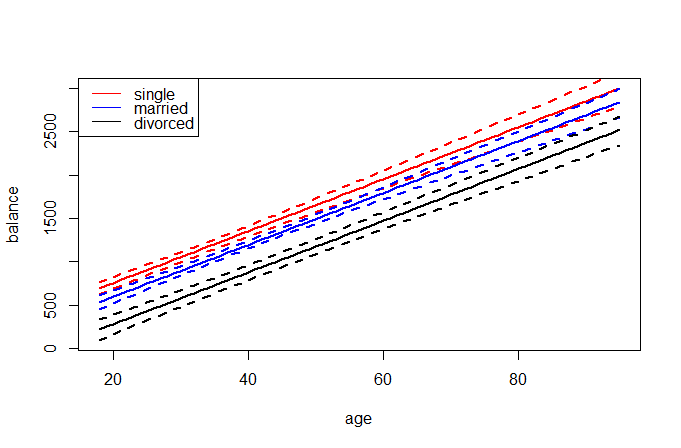
\includegraphics[width=0.8\textwidth]{intervals_h.png}
        \caption{Confidence interval of balance for contacts with housing loan\label{fig:intervals_h}}
    \end{figure}
     \begin{figure}[H]
    \centering
        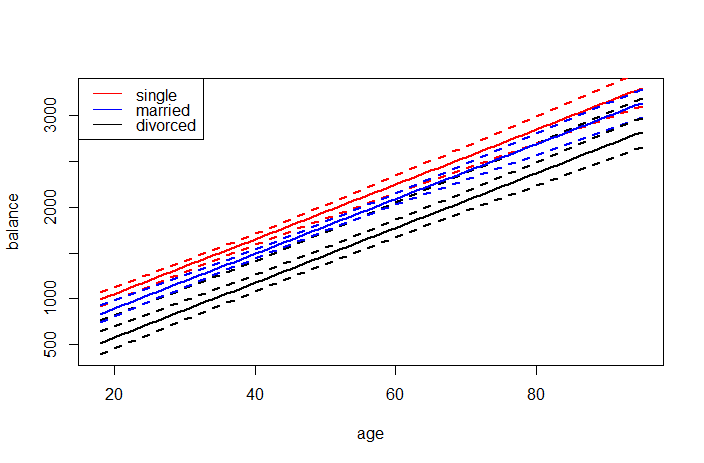
\includegraphics[width=0.8\textwidth]{intervals.png}
        \caption{Confidence interval of balance for contacts without housing loan\label{fig:intervals}}
    \end{figure}
    We see that for contacts of the same age and housing loan status, those who are single are expected to have higher balance than the married and the divorced. The expectation of balance for contacts who are divorced is the lowest among all three groups of marital status.\par
    For section \ref{2.2}, the MCMC draws of $\bm{z}$ is stored in the matrix \verb|Z2|. We can compute the proportion of $z_j$ such that $z_j = 1$ to approximate $Pr(z_j=1|\bm{y},\bm{X})$ for each $z_j$:
    \begin{verbatim}
> apply(Z2,2,mean)
[1] 1.0000 1.0000 0.9981 0.9981 0.0305 0.9547 0.0031 0.0031 0.0000
[10] 0.0000 0.0198 0.0198
    \end{verbatim}
    We see that the effects of \verb|age|, \verb|marital| and the interaction between \verb|age| and \verb|housing| are significant.\\
    It is noticed that for most coefficients the autocorrelations are high and the effective sample sizes are small:
    \begin{verbatim}
> apply(BETA2,2,effectiveSize)
[1]  1251.99824  4772.52507   524.25832   452.33426
[5]   923.18895   368.64501 17148.45635  6696.94495
[9]     0.00000     0.00000    72.80988    72.29301
    \end{verbatim}
    The MCMC diagnostic is not satisfactory as the small effective sample size and high autocorrelation show that the Gibbs sampler moves slowly around the parameter space. Reasons may include that many models with small probabilities are not sampled and the $z_j$ for some regressors(which have no effect) are always 0.\\
    We may also fit a model including all regressors and generate independent Monte Carlo samples from the posterior distribution of $\beta$ to compare the results:
\begin{verbatim}
> tmp<-lm.gprior3(y,X)
> beta.post<-tmp$beta
> apply(beta.post,2,function(x) quantile(x,c(0.025,0.975)))
                   age      m.single  m.married   h.yes    age_h.yes
2.5%  -1089.38195 26.60025  564.3378  -66.78193 -611.4643 -24.24718
97.5%    62.45592 50.07939 1856.9151 1204.91231  991.1351  10.87604
        age:m.single   age:m.married m.single:h.yes   m.married:h.yes
2.5%    -29.777365     -15.68529     -1269.0571       -930.2143
97.5%    -1.526961      10.04131       575.6694        866.8636
               age:m.single:h.yes  age:m.married:h.yes
2.5%           -18.27073           -23.17682
97.5%           24.39952            15.18380
\end{verbatim}
    We see that only for \verb|age|,\verb|m.single| (the dummy variable of \verb|marital| of the level \verb|single|), the 95\% confidence interval of the corresponding $\beta$ does not include 0, which supports our claim that the martial status has a significant effect on balance.
	\section{Conclusions}
	The main question of the project is whether the balance of contacts depends on their marital status. From what we did in section \ref{2.1} , \ref{2.2}, and the results shown in section \ref{results}, we notice that the \verb|marital| predictor does explain a large amount of variance.\\
    As suggested by the posterior mean and the confidence interval of $\bm{\beta}$, we conclude that for contacts of the same age and housing loan status, the expectation of balance for those who are married is higher than for those who are divorced, but lower than for those who are single.\\
    I would like to thank Dr Loong and Jiali for their valuable advice on the project. Doing the project makes me to be more familiar Monte Carlo sampling, Gibbs sampler, and basic Bayesian statistical methods including Bayesian model comparison, model averaging, etc. I've also practised the skills of report writing, R programming, and using \LaTeX.\\
    To extend the analysis of the dataset, I would consider including other variables as potential regressors. I would do more research on model diagnostics for regression to determine the most appropriate model for prediction and other purposes. I would explore other Bayesian computation methods to get more accurate and efficient approximation to the posterior distributions of the models and coefficients.
	\section{Self-Criticism\label{Self-Criticism}}
	While the dataset we use contains 17 variables, we only use 4 of them. Hence, the model we fitted may not have good performance for prediction(as we will have larger $\sigma^2$).\\ 
    Including small amount of predictors may also leads to misleading results. For example, if we only fit a simple linear regression using marital as the predictor and balance as response, we may find that the married may have the highest expected balance:
    \begin{verbatim}
> coef(lm(balance~marital))
(Intercept) maritalmarried  maritalsingle 
1178.8723       247.0533       122.6254 
    \end{verbatim}
    In our conclusion above, a contact who is single is expected to have higher balance than a married contact, if they are at same age and status of housing loan. This happens as the effect of marital status on age is significant.\\
    Therefore, if we can include more predictors, we may have better understandings of the relationships between the predictors, thus can propose more useful model to help the banking institution to make decisions.\\
    We may also examine the higher order terms of numeric predictors to expand our model space if we had more time.\\
    The Gibbs sampler used in \ref{2.2} takes more than 2 hours for 10000 iterations on my laptop due to large sample sizes. Further investigations may be required to accelerate the MCMC computation or we may need to explore alternatives as the effective sample sizes are small.\\
    In section \ref{results}, we plot the confidence interval of balance using the $11^{th}$ model. We may improve the analysis if we can find a way to compute the confidence interval using model averaged estimate of $\bm{\beta}$. Taking count into model uncertainty, the results we get may be more reliable than the results obtained simply by using the model with highest marginal posterior probability.
	\section{Appendices - R code for the project}
    \subsection{Setup and creating indicator variables}
    \begin{verbatim}
setwd("C:/Users/Ton/OneDrive/Document/STAT3016/Project")
bank<-read.csv("bank.csv",header =T,sep=";")
#attach(bank)
age<-bank$age
marital<-bank$marital
housing<-bank$housing
balance<-bank$balance

#create indicator variable for marital
m.married<-ifelse(marital=="married",1,0)
m.single<-ifelse(marital=="single",1,0)
marital.indicator<-cbind(m.single,m.married)

#indicator variable for housing
h.yes<-ifelse(housing=="yes",1,0)

#interaction term of housing and marital
marital_h.yes<-marital.indicator*h.yes
colnames(marital_h.yes)<-c("m.single:h.yes","m.married:h.yes")

#intercation between age and housing
age_h.yes<-age*h.yes

#interaction between age and marital
age.marital<-age*marital.indicator
colnames(age.marital)<-c("age:m.single","age:m.married")

#three-way interaction between age, marital, and housing
age.housing.marital<-age*marital_h.yes
colnames(age.housing.marital)<-c("age:m.single:h.yes",
    "age:m.married:h.yes")

#values of predictors
X<-cbind(rep(1,nrow(bank)),age,marital.indicator,h.yes,
age_h.yes,age.marital,marital_h.yes,age.housing.marital)
#values of the response variable
y<-balance

#check whether the dummy variables are created correctly
coef(lm(y~-1+X))
coef(lm(balance~age*housing*marital))
\end{verbatim}
\subsection{Bayesian model comparison}
\begin{verbatim}
#Bayesian model comparison

z<-matrix(data = rep(c(1,rep(0,11)),18), ncol = 12, byrow = T)

#Null model
z[1,]

#balance~age
z[2,2]<-1

#balance~marital
z[3,c(3,4)]<-1

#balance~house
z[4,c(4,5)]<-1

#balance~age+marital
z[5,c(2,3,4)]<-1

#balance~marital+house
z[6,c(3,4,5)]<-1

#balance~age+house
z[7,c(2,5)]<-1

#balance~age+marital+age:marital
z[8,c(2,3,4,7,8)]<-1

#balance~marital+house+marital:house
z[9,c(3,4,5,9,10)]<-1

#balance~age+house+age:house
z[10,c(2,5,6)]<-1

#balance~age+house+marital
z[11,c(2,3,4,5)]<-1

#balance~age+house+marital+age:house
z[12,c(2,3,4,5,6)]<-1

#balance~age+house+marital+age:marital
z[13,c(2,3,4,5,7,8)]<-1

#balance~age+house+marital+marital:house
z[14,c(2,3,4,5,9,10)]<-1

#balance~age+house+marital+age:house+age:marital
z[15,c(2,3,4,5,6,7,8)]<-1

#balance~age+house+marital+age:house+marital:house
z[16,c(2,3,4,5,6,9,10)]<-1

#balance~age+house+marital+age:marital+marital:house
z[17,c(2,3,4,5,7,8,9,10)]<-1

#balance~age+house+marital+age:marital+marital:house+
    age:house+age:marital:house
z[18,]<-rep(1,12)

lpy.X3<-function(y,X,
g=length(y),nu0=1,s20=try(summary(lm(y~-1+X))$sigma^2,silent=TRUE)) 
{
n<-dim(X)[1] ; p<-dim(X)[2] 
if(p==0) { s20<-mean(y^2) }
SS0<-t(y)%*%y-(g/(g+1))*(t(y)%*%X)%*%(solve(t(X)%*%X)%*%(t(X)%*%y))
-.5*n*log(2*pi) +lgamma(.5*(nu0+n)) - lgamma(.5*nu0)  - .5*p*log(1+g) +
.5*nu0*log(.5*nu0*s20) -.5*(nu0+n)*log(.5*(nu0*s20+SS0))
}

lm.gprior3<-function(y,X,g=dim(X)[1],nu0=1,
    s20=try(summary(lm(y~-1+X))$sigma^2,silent=TRUE),S=1000)
{

n<-dim(X)[1] ; p<-dim(X)[2]
SSRg<-t(y)%*%y-(g/(g+1))*t(y)%*%X%*%solve(t(X)%*%X)%*%(t(X)%*%y)

s2<-1/rgamma(S, (nu0+n)/2, (nu0*s20+SSRg)/2 )

Vb<- g*solve(t(X)%*%X)/(g+1)
Eb<- Vb%*%t(X)%*%y

E<-matrix(rnorm(S*p,0,sqrt(s2)),S,p)
beta<-t(  t(E%*%chol(Vb)) +c(Eb))

list(beta=beta,s2=s2)                                
}   

###  Marginal probabilities of the data under 18 different models  ###
lpy.p3<-NULL
for (i in 1:nrow(z))
{
z.use<-z[i,]
lpy.p3<-c(lpy.p3,lpy.X3(y,X[,z.use==1,drop=FALSE]))

}
#subtract mean(lpy.p) for computation stability
# pz<-NULL
# for(i in 1:length(lpy.p3)){
#   pz<-c(pz,round(1/sum(exp(lpy.p3-lpy.p3[i])),4))
# }
round(exp(-mean(lpy.p3)+lpy.p3)/sum(exp(-mean(lpy.p3)+lpy.p3)),4)
#post confidence intervals for beta.post
tmp<-lm.gprior3(y,X)
beta.post<-tmp$beta
apply(beta.post,2,function(x) quantile(x,c(0.025,0.975)))
apply(beta.post,2,mean)
\end{verbatim}
\subsection{Model averaging}
\begin{verbatim}
# Starting values and MCMC setup
z<-rep(1,ncol(X))#Starting value for z
BETA<-matrix(NA,S,ncol(X))
lpy.c<-lpy.X3(y[subset],X[subset,z==1,drop=FALSE])
S<-10000
Z<-matrix(NA,S,ncol(X))
#####

#####Gibbs sampler
###Takes long time
for(s in 1:S){
if(s%%100==0){cat(s,"\n")}
for(j in sample(2:dim(X)[2])){
zp<-z; zp[j]<-1-zp[j]
lpy.p<-lpy.X3(y,X[,zp==1,drop=FALSE])
r<-(lpy.p-lpy.c)*(-1)^(zp[j]==0)
z[j]<-rbinom(1,1,1/(1+exp(-r)))
if(z[j]==zp[j]){lpy.c<-lpy.p}
}
Z[s,]<-z
}
for(i in 1:nrow(Z)){
if(i%%100==0){cat(i,"\n")}
beta<-Z[i,]
beta[Z[i,]==1]<-lm.gprior3(y,X[,Z[i,]==1,drop=FALSE],S=1)$beta
BETA[i,]<-beta
}
apply(Z,2,mean)
apply(BETA,2,function(x) quantile(x,probs=c(0.025,0.975)))

##to be grouped
g<-list(2,c(3,4),5,6,c(7,8),c(9,10),c(11,12))
z<-rep(1,ncol(X))
lpy.c<-lpy.X3(y,X[,z==1,drop=FALSE])
S<-10000
Z2<-matrix(NA,S,ncol(X))
BETA2<-matrix(NA,S,ncol(X))
#####

#####Gibbs sampler
for(s in 1:S){
if(s%%100==0){cat(s,"\n")}
for(j in sample(1:length(g))){
zp<-z; zp[g[[j]]]<-1-zp[g[[j]]]
lpy.p<-lpy.X3(y,X[,zp==1,drop=FALSE])
r<-(lpy.p-lpy.c)*(-1)^(zp[g[[j]]][1]==0)
z[g[[j]]]<-rep(rbinom(1,1,1/(1+exp(-r))),length(g[[j]]))
if(z[g[[j]]][1]==zp[g[[j]]][1]){lpy.c<-lpy.p}
}
Z2[s,]<-z
}

for(i in 1:nrow(Z2)){
if(i%%100==0){cat(i,"\n")}
beta<-Z2[i,]
beta[Z2[i,]==1]<-lm.gprior3(y,X[,Z2[i,]==1,drop=FALSE],S=1)$beta
BETA2[i,]<-beta
}
apply(Z2,2,mean)
apply(BETA2,2,function(x) quantile(x,probs=c(0.025,0.975)))
apply(BETA2,2,function(x) mean(x!=0))
library(coda)
apply(BETA2,2,effectiveSize)
for(i in 1:ncol(BETA2)){
acf(BETA2[,i]) #error as some z's are always 0
}
\end{verbatim}
\subsection{Confidence interval}
\begin{verbatim}
##### plot the confidence interval
age.seq<-18:95
n.age<-length(age.seq)
z11<-c(rep(1,5),rep(0,7))
beta.post11<-lm.gprior3(y,X[,z11==1])$beta
balance.single.h<-balance.married.h<-balance.divorced.h<-NULL
balance.single<-balance.married<-balance.divorced<-NULL
for (i in 1: n.age){
balance.single.h<-rbind(balance.single.h,
quantile(beta.post11[,1]+beta.post11[,2]*age.seq[i]
+beta.post11[,3]+beta.post11[,5],prob=c(0.025,0.5,0.975)))
balance.married.h<-rbind(balance.married.h,
    quantile(beta.post11[,1]+beta.post11[,2]*age.seq[i]
    +beta.post11[,4]+beta.post11[,5],prob=c(0.025,0.5,0.975)))
balance.divorced.h<-rbind(balance.divorced.h,
    quantile(beta.post11[,1]+beta.post11[,2]*age.seq[i]
    +beta.post11[,5],prob=c(0.025,0.5,0.975)))
balance.single<-rbind(balance.single,
    quantile(beta.post11[,1]+beta.post11[,2]*age.seq[i]
    +beta.post11[,3],prob=c(0.025,0.5,0.975)))
balance.married<-rbind(balance.married,
    quantile(beta.post11[,1]+beta.post11[,2]*age.seq[i]
    +beta.post11[,4],prob=c(0.025,0.5,0.975)))
balance.divorced<-rbind(balance.divorced,
    quantile(beta.post11[,1]+beta.post11[,2]*age.seq[i]
    ,prob=c(0.025,0.5,0.975)))
}

#plot 1: with housing loan
intervals.h<-list(balance.single.h,balance.married.h,balance.divorced.h)
colors3<-c("red","blue","black")
plot(age.seq,balance.single.h[,3],type="l",lwd=2,lty=2,ylim=
c(min(c(balance.divorced.h[,1],balance.married.h[,1],
    balance.divorced.h[,1])),
max(c(balance.divorced.h[,3],balance.married.h[,3],
    balance.divorced.h[,3]))),
ylab="balance",xlab="age")
for(i in 1:length(intervals.h)){
lines(age.seq,intervals.h[[i]][,1],type="l",lwd=2,lty=2,col = colors3[i])
lines(age.seq,intervals.h[[i]][,2],type="l",lwd=2,lty=1,col = colors3[i])
lines(age.seq,intervals.h[[i]][,3],type="l",lwd=2,lty=2,col = colors3[i])
}
legend("topleft",c("single","married","divorced"),lty=1,col=colors3)

#plot 2: no housing loan
intervals<-list(balance.single,balance.married,balance.divorced)
plot(age.seq,balance.single.h[,3],type="l",lwd=2,lty=2,ylim=
c(min(c(balance.divorced[,1],balance.married[,1],balance.divorced[,1])),
max(c(balance.divorced[,3],balance.married[,3],balance.divorced[,3]))),
ylab="balance",xlab="age")
for(i in 1:length(intervals)){
lines(age.seq,intervals[[i]][,1],type="l",lwd=2,lty=2,col = colors3[i])
lines(age.seq,intervals[[i]][,2],type="l",lwd=2,lty=1,col = colors3[i])
lines(age.seq,intervals[[i]][,3],type="l",lwd=2,lty=2,col = colors3[i])
}
legend("topleft",c("single","married","divorced"),lty=1,col=colors3)


coef(lm(balance~marital))
lm(age~marital)

    \end{verbatim}
    
	\begin{thebibliography}{9}
		\bibitem{faraway}
		Julian J. Faraway.
		\textit{Linear Models with R}.
		CRC Press, Boca Raton, 2014
		\bibitem{hoff}
        Peter D. Hoff.
        \textit{A First Course in Bayesian Statistical Methods}.
        University of Washington, Seattle, 2010
	\end{thebibliography}
\end{document}